\documentclass[aspectratio=169]{beamer}

\usepackage[utf8]{inputenc}
\usepackage[T1]{fontenc}
\usepackage{lmodern}
\usepackage{amsmath}
\usepackage{amssymb}
\usepackage{graphicx}
\usepackage{booktabs}
\usepackage{tikz}
\usetikzlibrary{positioning, arrows.meta, shapes.geometric}
\usepackage{tcolorbox}

\usetheme{Madrid}
\usecolortheme{default}
\useinnertheme{circles}
\usefonttheme{professionalfonts}

\setbeamerfont{author in head/foot}{size=\fontsize{6}{7}\selectfont}
\setbeamerfont{title in head/foot}{size=\fontsize{6}{7}\selectfont}
\setbeamerfont{date in head/foot}{size=\fontsize{5}{6}\selectfont}

\title[Optimization of an ADS]{Maximization of the operational multiplication factor in a photon driven subcritical reactor: a methodological approach for temperature and poison feedback}

\author[R. Bossi]{
  Riccardo Bossi \\ \medskip
  {\small Supervisor: Prof.ssa Monica Sisti} \\
  {\small Co-supervisor: Prof. Antonio Cammi}
}

\institute[Bicocca \& PoliMi]{University of Milano-Bicocca \\ Politecnico of Milano}
\date{6/07/2026}

\titlegraphic{%
  \vspace{-3cm} % Modifica questo valore per regolare l'altezza
  \centering
  
\includegraphics[height=2.5cm]{logo_bicocca.png}%
  \hspace{8cm}% Spazio orizzontale tra i due loghi
  \includegraphics[height=2.5cm]{logo_polimi.png}%
}

\begin{document}

% === SLIDE 1: TITOLO ===
\begin{frame}
  \titlepage
\end{frame}


% === SLIDE 2: CONTESTO E OBIETTIVO ===
\begin{frame}{Thesis Context and Objective}
    \begin{block}{Subcritical System}
        A reactor with $k_{eff} < 1$ requires an \textbf{external neutron source} to sustain the chain reaction. The power is proportional to the source intensity, but \textbf{feedbacks} modify $k_{eff}$ during transients.
    \end{block}
    
    \vspace{0.5cm}
    
    \begin{alertblock}{Objective}
        Develop a methodology to \textbf{maximize} $k_{eff}^{HFP}$ (deeply linked to power production) ensuring that $k_{eff}^{CZP} \leq 1$ under any operating condition.
    \end{alertblock}
    
    \vspace{0.3cm}
    
    \begin{itemize}
        \item \textbf{CZP} (Cold Zero Power): $T = 300$ K — reactor shutdown
        \item \textbf{HFP} (Hot Full Power): $T_{fuel} = 600$ K, $T_{mod} = 350$ K — nominal operation 
    \end{itemize}
\end{frame}

% === SLIDE 3: PROGETTO SYNERGY ===
\begin{frame}{SYNERGY Project: Photonic Source}

    To overcome the limitations of accelerator based neutron sources — specifically the excessive heat deposition of charged particles on the converter — this thesis is developed within the SYNERGY project:
    \begin{columns}[c]
        \begin{column}{0.55\textwidth}
            \begin{itemize}
                \item Synchrotron-based neutron source utilizing extracted $\gamma$-photons (1–37 MeV) to mitigate thermal load on the converter
                \item Photonuclear $(\gamma, xn)$ reactions and photofission $(\gamma, f)$ on a natural Uranium target
                \item Photonic rate: $S_\gamma = 2.02 \times 10^{17}$ $\gamma$/s
                \item Neutronic rate up to $10^{15}$ n/s
                \item Beam power: $\sim 200$ kW per beamline
            \end{itemize}
        \end{column}
        \begin{column}{0.45\textwidth}
            \vspace{0.2cm}
            \centering
            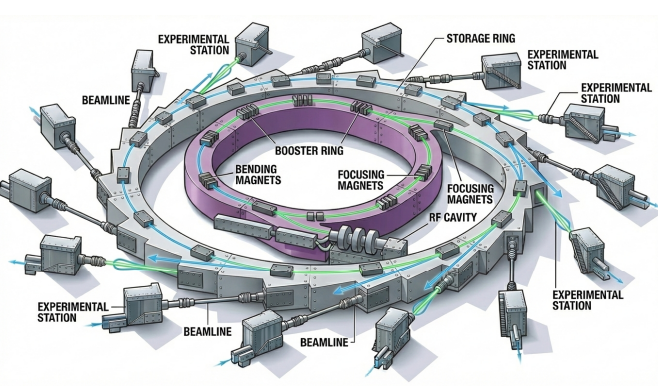
\includegraphics[width=\textwidth]{Sincrotrone_anello.png}
        \end{column}
    \end{columns}
\end{frame}

\begin{frame}{From Source to Core: The Physical Workflow}
    
    \vspace{0.2cm}
    \centering
    % Inserisci qui il nome del file dell'immagine dello schema a blocchi
    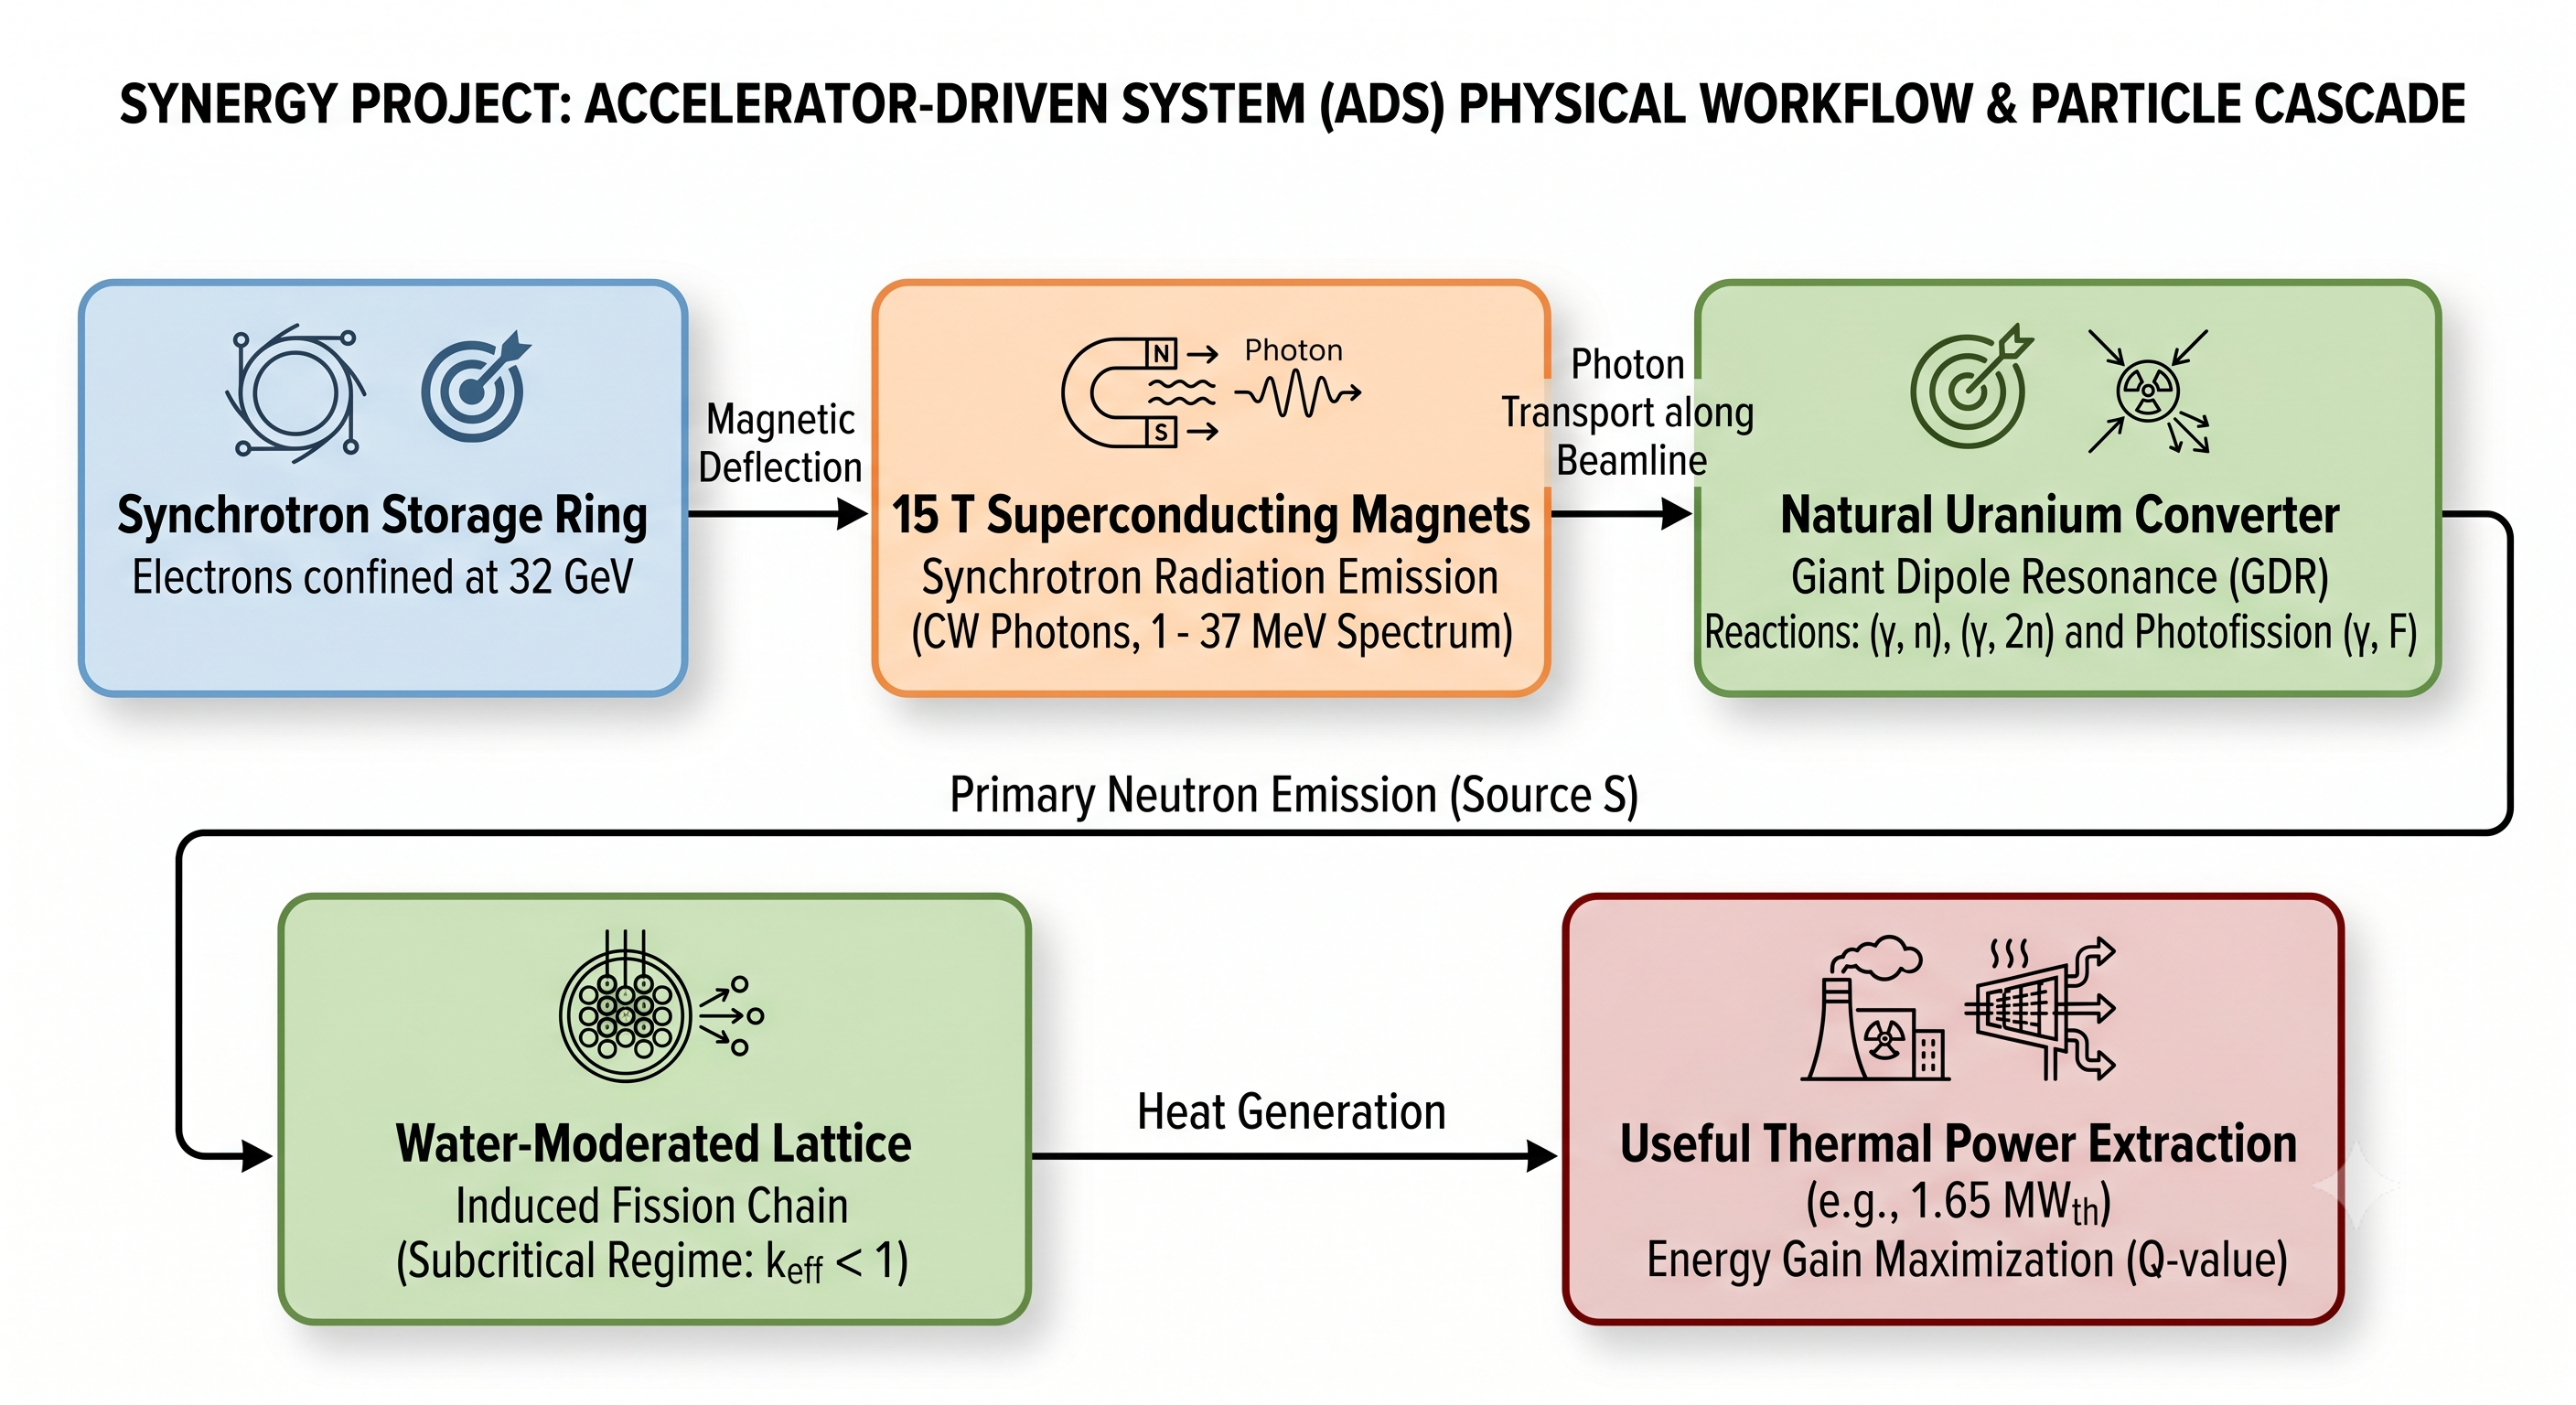
\includegraphics[width=0.85\textwidth]{work_flow.png} 
    
    \vspace{0.1cm}
    
    \begin{columns}[c]
        \begin{column}{0.9\textwidth}
            \begin{itemize}
                \item The \textbf{photoneutrons} generated in the central target act as the external driving source ($S$) for the surrounding subcritical core.
                \item The multiplied neutron flux generates thermal power, which in turn alters the \textbf{thermodynamic state} of the system.
            \end{itemize}
        \end{column}
    \end{columns}
\end{frame}

% === SLIDE 4: FEEDBACK DI REATTIVITÀ ===
\begin{frame}{Reactivity Feedbacks}

    During the transition from HFP to CZP, the temperature drop induces a \textbf{reactivity insertion}. The primary feedback mechanisms are: \\
    \vspace{0.3cm}
    \begin{columns}[T]
        \begin{column}{0.6\textwidth}
            \textbf{Doppler Effect}
            \begin{itemize}
                \item Narrowing of $^{238}$U capture resonances due to reduced thermal agitation
                \item Decreased epithermal absorption $\Rightarrow$ \textcolor{red}{$\Delta\rho > 0$}
            \end{itemize}
            
            \vspace{0.5cm}
            
            \textbf{Moderator Effect}
            \begin{itemize}
                \item Increase in water density as temperature decreases
                \item Enhanced neutron thermalization $\Rightarrow$ \textcolor{red}{$\Delta\rho > 0$}
            \end{itemize}
        \end{column}
        
        \begin{column}{0.4\textwidth}
            \begin{alertblock}{Reactivity Variation}
                \begin{equation*}
                    \Delta\rho = \frac{k_2 - k_1}{k_1 \cdot k_2} \quad \text{ [pcm]}
                \end{equation*}
            \end{alertblock}
            
            \vspace{0.3cm}
            
            \begin{block}{Safety Constraint}
                \begin{equation*}
                    k_{max}^{HFP} =  k_{max}^{CZP} - \sum_i \Delta\rho_i
                \end{equation*}
            \end{block}
        \end{column}
    \end{columns}
\end{frame}

% === SLIDE 7: CORE TOPOLOGY & FUEL ZONING ===
\begin{frame}{Core Topology and Variable Enrichment}
    \begin{columns}[T]
        \begin{column}{0.48\textwidth}
            \vspace{0.5cm}
            \centering
            
\includegraphics[width=0.95\textwidth]{reactor_xy_v.png}
            
            \vspace{0.2cm}
            \footnotesize \textit{Hexagonal Lattice (XY Section)}
        \end{column}
        
        \begin{column}{0.5\textwidth}
            \begin{block}{Core Materials}
                \begin{itemize}
                    \item \textbf{Fuel:} $UO_2$ pins with Zirconium cladding.
                    \item \textbf{Moderator:} Light water doped with 15\% heavy water ($H_2O$ + 15\% $D_2O$).
                    \item \textbf{Reflector:} Nuclear graphite.
                \end{itemize}
            \end{block}
            
            \vspace{0.1cm}
            
            \begin{alertblock}{Enrichment Strategy (Fuel Zoning)}
                \textbf{Radial linear profile:} $^{235}U$ enrichment varies from the inner rings towards the core periphery.
            \end{alertblock}
            
            \vspace{0.1cm}
            
        \end{column}
    \end{columns}
\end{frame}

% === SLIDE 5: SUPERFICIE k(T) ===
\begin{frame}{Thermodynamic Multiplication Surface}
    \begin{columns}[c]
        \begin{column}{0.5\textwidth}
            \centering
            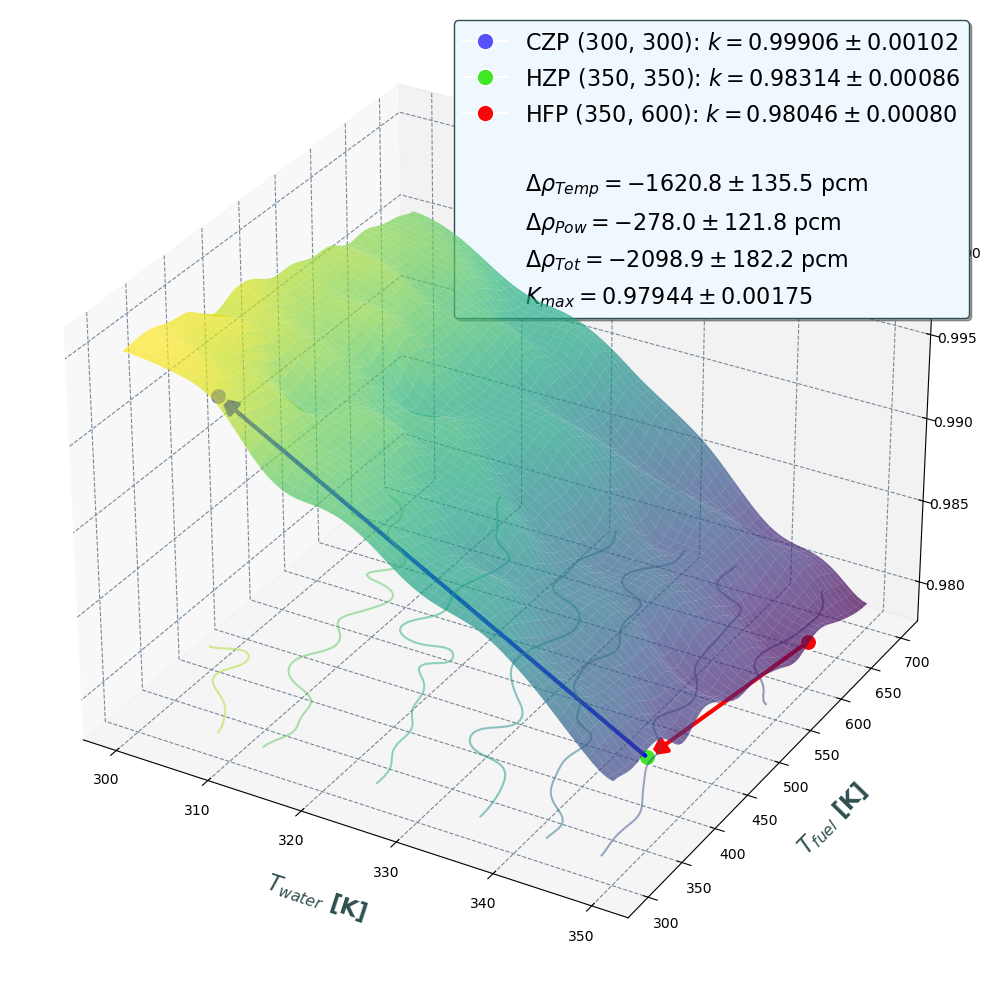
\includegraphics[width=\textwidth]{superficie.png}
        \end{column}
        \begin{column}{0.45\textwidth}
            \footnotesize
            3D map of $k_{eff}(T_{fuel}, T_{mod})$ in the HFP $\rightarrow$ HZP $\rightarrow$ CZP transient.
            
            \vspace{0.5cm}
            
            The system cooling causes a \textbf{reactivity increase} that must be compensated by the initial subcriticality margin.\\

            In addition, another 200 pcm are added as a safety margin to account for uncertainties in the feedback quantification.
            
            \begin{block}{Pitch optimization}
                Keeping the operating temperatures fixed, what is the optimal pitch to maximize $k_{max}$ ?
            \end{block}
        \end{column}
    \end{columns}
\end{frame}

% === SLIDE 6: OTTIMIZZAZIONE DEL PITCH ===
\begin{frame}{Lattice Pitch Optimization}
    Pitch governates the moderation level and the neutron spectrum, thus affecting the multiplication factor
    \begin{columns}[c]
        \begin{column}{0.6\textwidth}
            \centering
            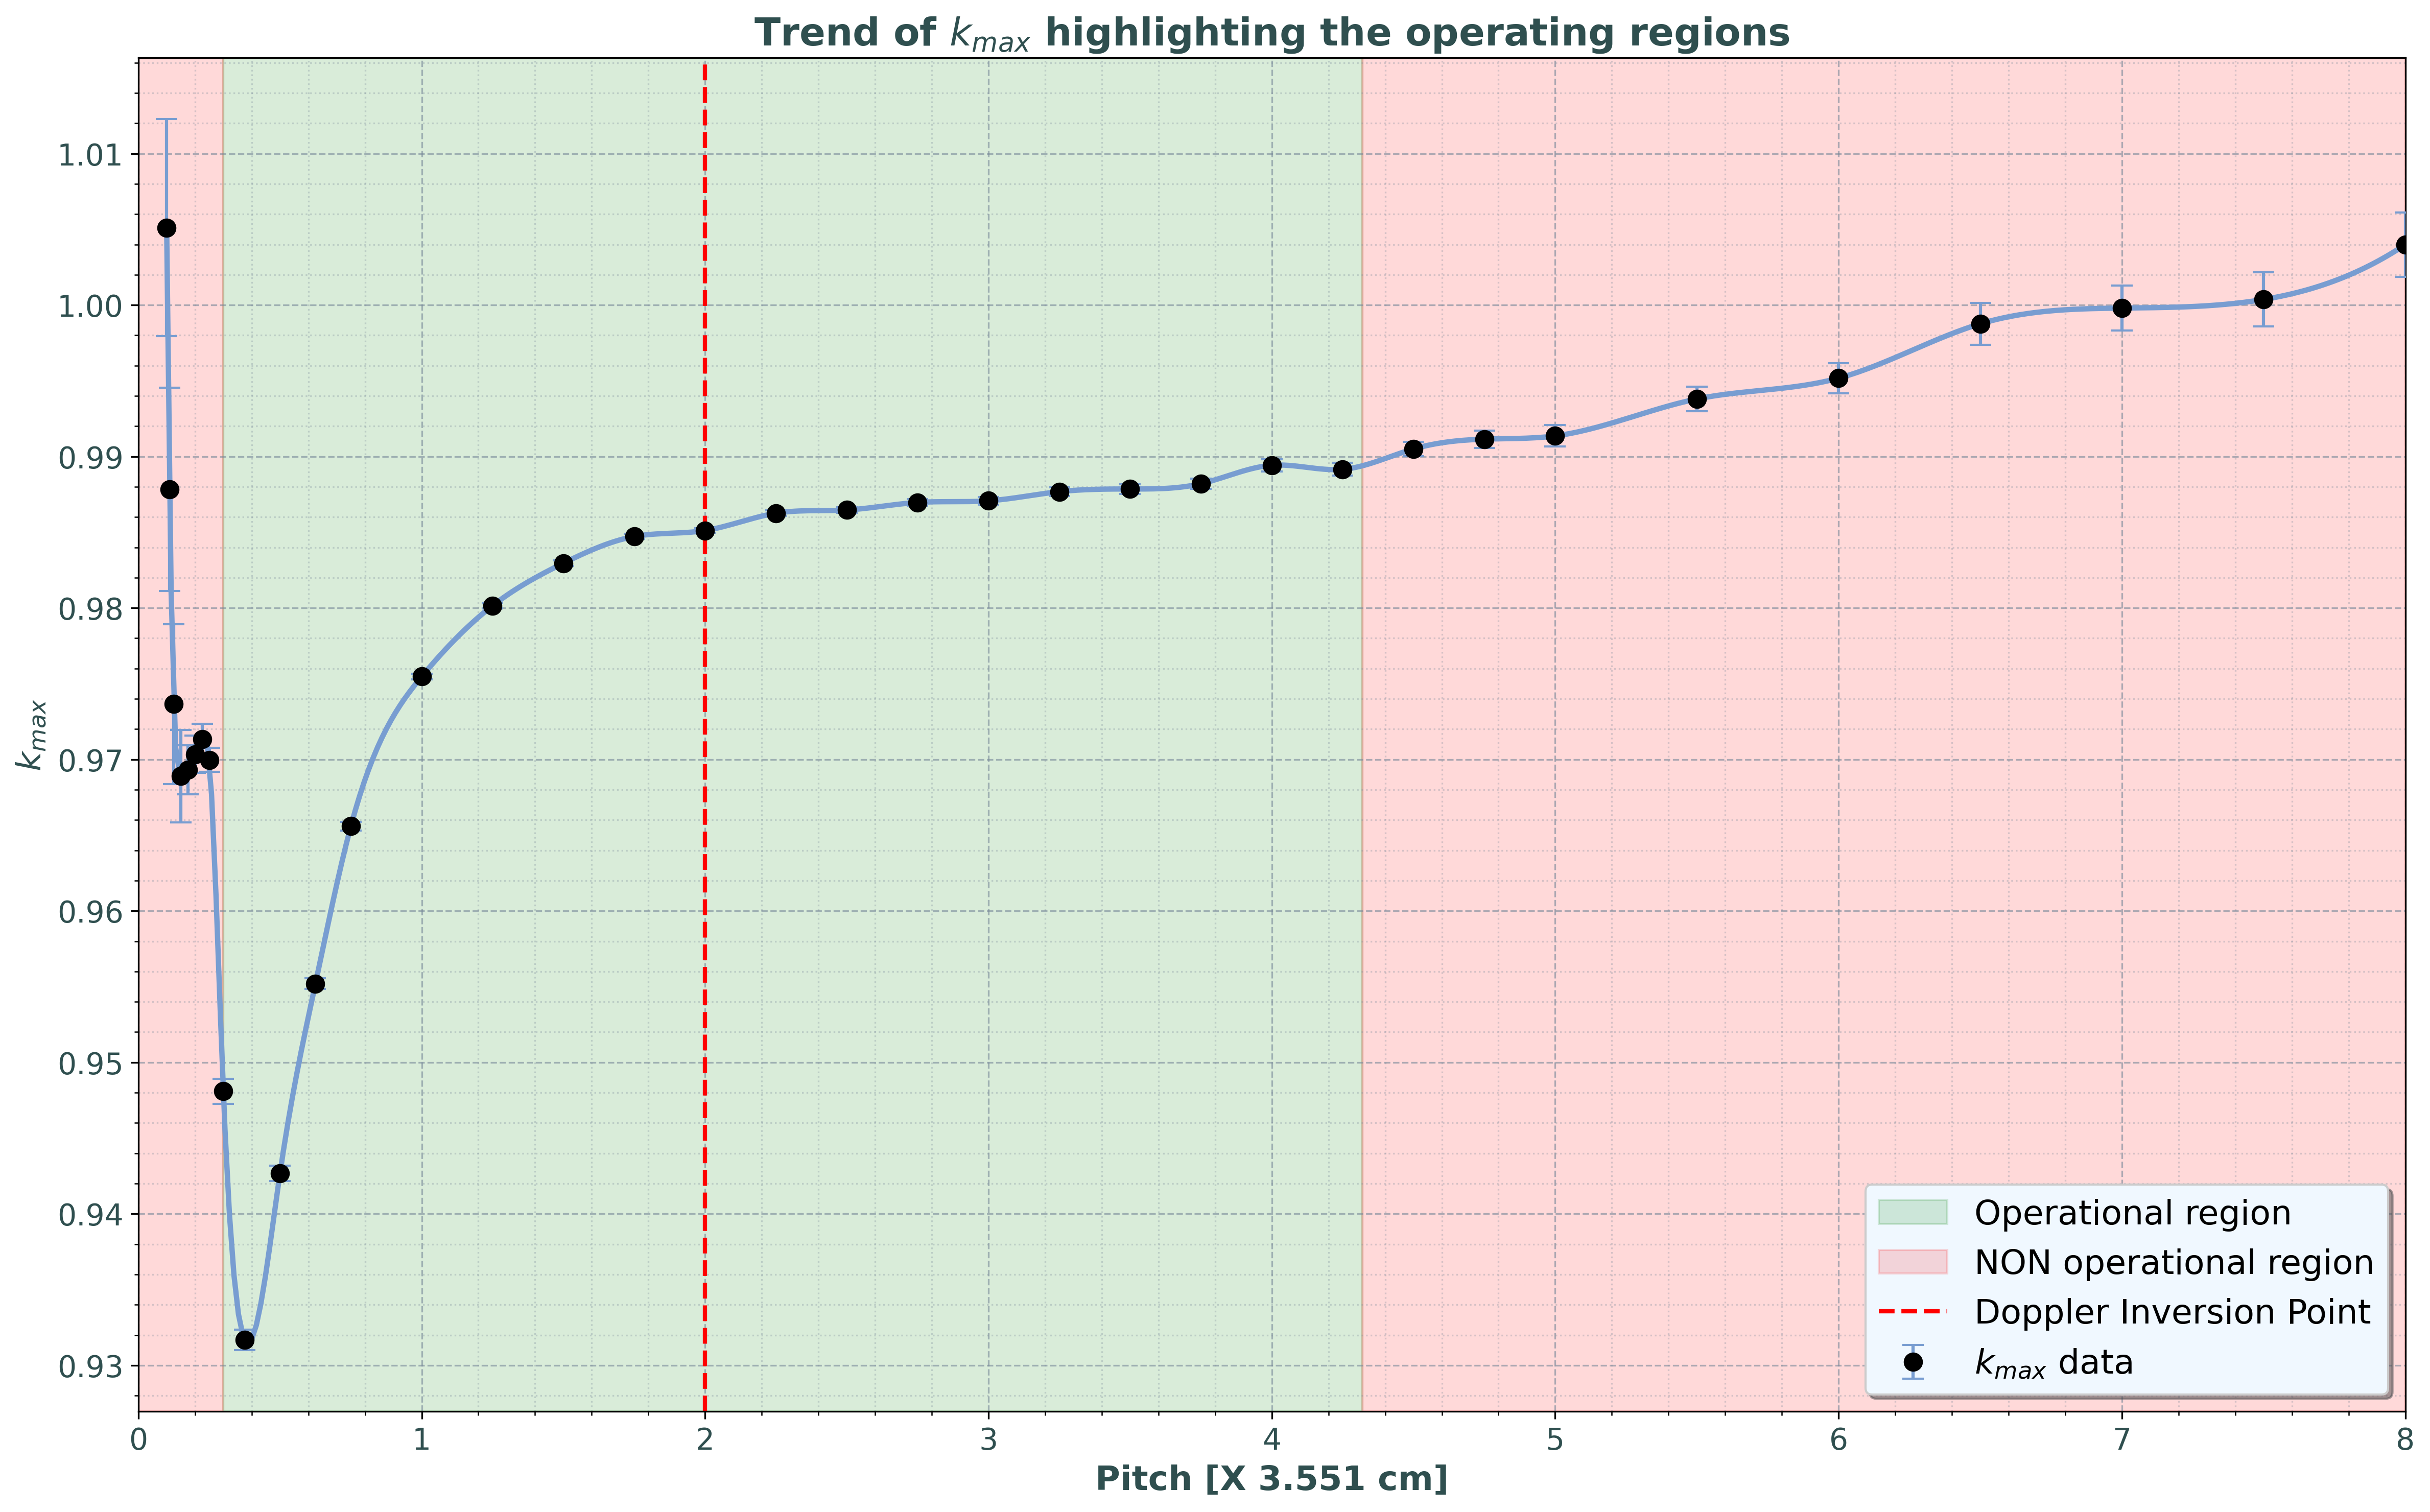
\includegraphics[width=\textwidth]{operatività.png}
        \end{column}
        \begin{column}{0.4\textwidth}
            \begin{itemize}
                \item \textbf{Green Zone:} Possible operation — target $k_{max}$ reachable by modulating enrichment
                \item \textbf{Red Zone:} Inaccessible — target not reached even at 100\% enrichment
                \item Important to emphatized that over multiplication pitch of 2 \textbf{the doppler effect inverts sign}, meaning that the reactore is instable at source oscillation 
            \end{itemize}
        \end{column}
    \end{columns}
\end{frame}


% === SLIDE 8: RISULTATI POTENZA ===
\begin{frame}{Results: Power and Multiplication vs. Pitch}
    \begin{columns}[c]
        \begin{column}{0.65\textwidth}
            \centering
            
\includegraphics[width=\textwidth]{potenza_vs_pitch_zone.png}
        \end{column}
        
        \begin{column}{0.35\textwidth}
            \centering
            \textbf{Global Maximum}
            \begin{itemize}
                \item Pitch $\approx 14$ cm
                \item $P_{th} = 2.38$ MW
                \item \textcolor{red}{\textbf{Impractical}} for Doppler inversion
            \end{itemize}
            
            \rule{\linewidth}{0.4pt}
            \vspace{0.05cm}
            
            \centering
            \textbf{Feasible Maximum}
            \begin{itemize}
                \item Pitch $\approx 7$ cm
                \item $P_{th} = 1.65$ MW
                \item \textbf{Stable and safe}
                \item $Q$-Value = 4.12
            \end{itemize}
        \end{column}
    \end{columns}
\end{frame}

% === SLIDE 9: VELENI - TEORIA ===
\begin{frame}{Neutron Poisons: Xe-135 and Sm-149}
    Other than the thermal feedbacks, the presence of neutron poisons (fission products with high absorption cross section) can significantly reduce $k_{eff}$ during operation. The main poisons in a uranium-fueled reactor are:
    \vspace{0.3cm}
    \begin{columns}[T]
        \begin{column}{0.48\textwidth}
            \textbf{Xenon-135}
            \begin{itemize}
                \item $\sigma_a \approx 2 \times 10^6$ b
                \item Transient: \textbf{post-shutdown peak}
                \item Decays with $T_{1/2} = 9.2$ h
            \end{itemize}
            
            \begin{equation*}
                N_{Xe}^{eq} = \frac{(\gamma_I + \gamma_{Xe}) \Sigma_f \phi}{\lambda_{Xe} + \sigma_a \phi}
            \end{equation*}
        \end{column}
        
        \begin{column}{0.48\textwidth}
            \textbf{Samarium-149}
            \begin{itemize}
                \item $\sigma_a \approx 4.1 \times 10^4$ b
                \item \textbf{Stable} ($\lambda_{Sm} = 0$)
                \item Permanent asymptotic buildup
            \end{itemize}
            
            \begin{equation*}
                N_{Sm}^{eq} = \frac{\gamma_{Pm} \Sigma_f}{\sigma_{a,Sm}}
            \end{equation*}
            
        \end{column}
    \end{columns}
\end{frame}

% === SLIDE 10: SIMULAZIONI DEPLETION ===
\begin{frame}{Burnup Simulations: Poison Evolution}

    From the analytical resolution of the Bateman equations, it is possible to observe the behavior as the flux varies:
    \vspace{0.2cm}
    \begin{columns}[c]
        \begin{column}{0.5\textwidth}
            \centering
            
\includegraphics[width=\textwidth]{xenon_transient_analysis.png}
            
            \footnotesize Xe-135: post-shutdown peak
        \end{column}
        \begin{column}{0.5\textwidth}
            \centering
            
\includegraphics[width=\textwidth]{samarium_buildup_analysis.png}
            
            \footnotesize Sm-149: asymptotic plateau
        \end{column}
    \end{columns}
\end{frame}

% === SLIDE 11: EVOLUZIONE k_eff ===
\begin{frame}{Evolution of $k_{eff}$ over the Life Cycle}
    \begin{columns}[c]
        \begin{column}{0.55\textwidth}
            \centering
            
\includegraphics[width=\textwidth]{k_eff_zoom_1_000.png}
        \end{column}
        \begin{column}{0.43\textwidth}
            \footnotesize
            The post-shutdown $k_{eff}$ evolution is driven by the net reactivity balance of neutron poisons:
            
            \vspace{0.2cm}
            \begin{itemize}
                \item \textbf{Xenon-135} decays entirely without a transient peak, releasing positive reactivity.
                \item \textbf{Samarium-149} asymptotically accumulates, introducing a negative reactivity penalty.
            \end{itemize}
            \vspace{0.2cm}
            
            Since the positive reactivity gained from Xenon's disappearance strictly outweighs the Samarium penalty, the system experiences a \textbf{net reactivity gain}, leading to the asymptotic growth of the fundamental eigenvalue.
            
        \end{column}
    \end{columns}
\end{frame}


\begin{frame}{Poisoning Reactivity vs Pitch}
    \vspace*{-0.5cm} 
    \begin{figure}
        \centering
        
\includegraphics[width=0.85\textwidth, height=0.65\textheight, keepaspectratio]{poison_VS_pitch.png}
        
        \vspace{0.3cm} 
        
        \begin{minipage}{0.9\textwidth}
            \scriptsize
            \textbf{Figure:} Evolution of $\Delta\rho_{\text{Poison}}$ as the Pitch varies. The analysis highlights the absence of a global optimum, identifying instead a limiting condition ("worst-case") near the x2 multiplier.
        \end{minipage}
    \end{figure}
\end{frame}

\begin{frame}{Total Reactivity Balance}

    \begin{equation*}
        \Delta\rho_{tot} = \Delta\rho_{Doppler} + \Delta\rho_{Mod} + \Delta\rho_{Poison} + \Delta\rho_{Safety}
    \end{equation*}

    \vspace{0.3cm}

    \begin{columns}[c]
        \begin{column}{0.45\textwidth}
            \begin{table}
                \centering
                {\small \textbf{Lattice Pitch: $3.55 \text{ cm}$}} \\[0.15cm]
                \begin{tabular}{lc}
                    \toprule
                    \textbf{Contribution} & \textbf{[pcm]} \\
                    \midrule
                    Doppler & 417 \\
                    Moderator & 1897 \\
                    Poisons & 424 \\
                    Safety & 200 \\
                    \midrule
                    \textbf{Total} & \textbf{2938} \\
                    \bottomrule
                \end{tabular}
            \end{table}
        \end{column}
        
        \begin{column}{0.5\textwidth}
            \begin{alertblock}{Operational Limit}
                \begin{equation*}
                    k_{max}^{HFP} = 1 - 2938 \text{ pcm} = \boxed{0.97062}
                \end{equation*}
            \end{alertblock}
            
            \vspace{0.2cm}
            
            \footnotesize Below this limit, safety is guaranteed in any thermal transient. 
        \end{column}
    \end{columns}
\end{frame} 

% Slide 2: K_max vs Pitch
\begin{frame}{HFP Operability vs Pitch}
    \vspace*{-0.5cm} 
    \begin{figure}
        \centering
        
\includegraphics[width=0.85\textwidth, height=0.75\textheight, keepaspectratio]{K_MASSIMO.png}
        
        \vspace{0.3cm}
        
        \begin{minipage}{0.9\textwidth}
            \scriptsize
            \textbf{Figure:} Maximum $k_{\text{eff}}$ value in HFP regime as the pitch varies. The trend shows a constant improvement towards pitch x4, where the highest available safe multiplication value is achieved.
        \end{minipage}
    \end{figure}
\end{frame}

% === SLIDE 13: RISULTATI PRINCIPALI ===
\begin{frame}{Conclusion}
    \begin{columns}[T]
        \begin{column}{0.48\textwidth}
            \begin{block}{Methodological Framework}
                \begin{itemize}
                    \item \textbf{Parametric} and modular optimization procedure.
                    \item \textbf{Intrinsically agnostic}: easily adaptable to any alternative reactor layout (geometry, fuel, reflector, or moderator).
                \end{itemize}
            \end{block}
        \end{column}
        
        \begin{column}{0.48\textwidth}
            \begin{alertblock}{Quantitative Output vs. Lattice Pitch}
                \begin{itemize}
                    \item Maximum allowable operational eigenvalue ($k_{\text{HFP}}^{\text{max}}$).
                    \item Extracted thermal power and \textit{Q-value}.
                    \item Doppler, moderator density, and poisoning reactivity feedbacks.
                \end{itemize}
            \end{alertblock}
        \end{column}
    \end{columns}
    
    \vspace{0.5cm}
    
    \begin{block}{Original Contribution}
        First systematic quantification of the \textbf{total reactivity load} in a photon-driven ADS system through fully coupled Monte Carlo and depletion simulations (OpenMC + CRAM).
    \end{block}
\end{frame}

% === SLIDE 14: SVILUPPI FUTURI ===
\begin{frame}{Future Developments}
    \begin{itemize}
        \item \textbf{Thermal-Hydraulic Coupling:} 3D spatial integration between OpenMC and CFD/sub-channel solvers for exact local temperature gradient evaluation.
        \item \textbf{Dynamic Beam Control:} Implementation of a feedback control loop on the photon source intensity $S(t)$ to compensate for poison accumulation and maintain a constant thermal power.
        \item \textbf{Source Kinematic Refinement:} Integration of the real anisotropic angular distributions (peaked at $90^\circ$ for GDR) of the photoneutron emission.
        \item \textbf{Fast Spectrum Extension:} Application of the framework to a fast ADS core (Lead/LBE cooled) to optimize Minor Actinides (MA) transmutation.
    \end{itemize}
\end{frame}

% === SLIDE 15: CHIUSURA ===
\begin{frame}[plain, c]
    \centering
    \vspace{1.5cm}
    
    {\huge \textbf{Thank you for your attention!}}
    
    \vspace{1.5cm}
    
    {\Large \textit{Questions?}}
\end{frame}






\begin{frame}{Geometria ad Arricchiemnto variabile}
\begin{figure}
        \centering
      
        \begin{minipage}{0.48\textwidth}
            \centering
            
\includegraphics[width=0.9\linewidth]{reactor_xy_v.png}
            \caption{Sezione piano XY.}
        \end{minipage}
        \begin{minipage}{0.48\textwidth}
            \centering
            
\includegraphics[width=0.75\linewidth]{reactor_xz_v.png} % Larghezza ridotta per compensare l'altezza
            \caption{Sezione piano XZ.}
        \end{minipage}
    \end{figure}

    
\end{frame}

\begin{frame}{Spazio delle Soluzioni Stabili per un Pitch di 3.551 cm}
    \begin{figure}
        \centering
        
\includegraphics[width=0.78\textwidth]{regressione_parabolica_filtrata.png}
        \caption{ Locus dei punti di lavoro stabili}
        \label{fig:stabilità}
    \end{figure}
\end{frame}

\begin{frame}{Spazio delle Soluzioni Stabili}
    \begin{figure}
        \centering
        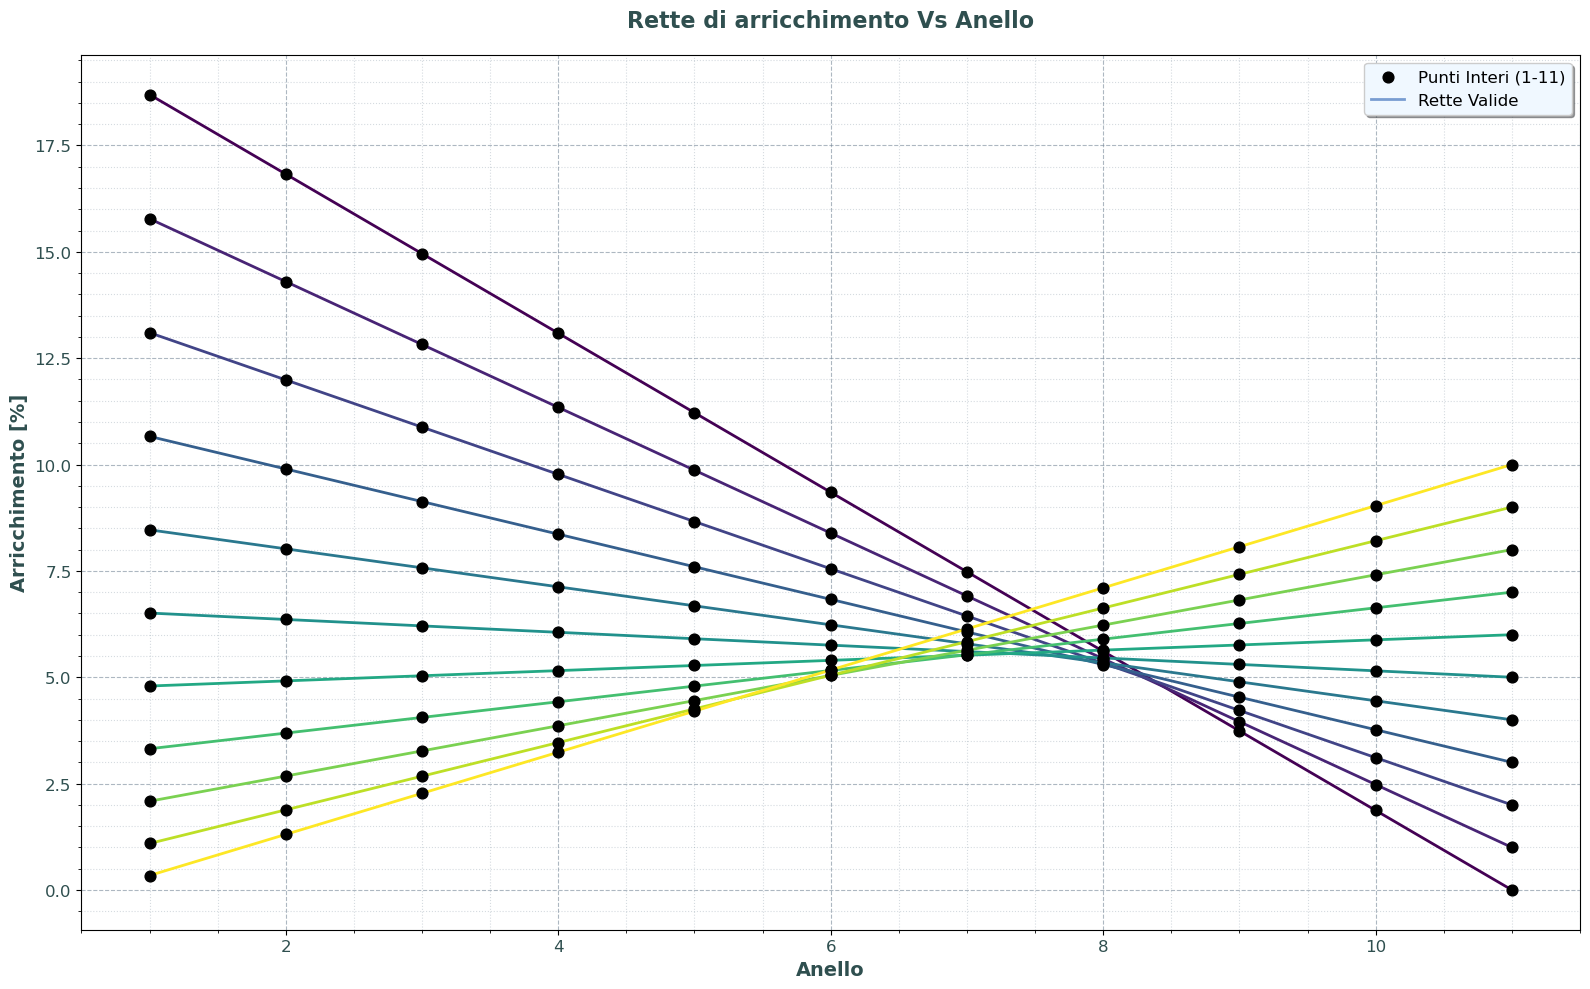
\includegraphics[width=0.68\textwidth]{rette_di_arricchimento.png}
        \caption{estrapolazione radiale per il gradiente di arricchimento.}
        \label{fig:stabilità2}
    \end{figure}
I punti di lavoro della slide precedente sono trovati con questa distribuzione radiale di arricchimenti
\end{frame}


\begin{frame}{Variazione della Potenza Estratta}
    \begin{figure}
        \centering
        
\includegraphics[width=0.7\textwidth]{scatter_potenza_errore.png}
        \caption{ Sensibilità della potenza termica macroscopica in funzione del grado di arricchimento radiale all'anello esterno}
        \label{fig:potenze}
    \end{figure}
\end{frame}


\begin{frame}{Parametri Prestazionali: Il Q-Factor}
    
    In un sistema ADS, il fattore di guadagno energetico $Q$ descrive l'amplificazione della potenza della sorgente nel nocciolo sottocritico:
    \begin{equation*}
        Q = \frac{P_{thermal}}{P_{beam}} = \psi \frac{k_{eff}}{1 - k_{eff}}
    \end{equation*}
    Dove $\psi$ rappresenta il fattore di importanza relativa dei neutroni di sorgente.
    
    Per una valutazione coerente si definisce un $Q_{sys}$ riferito alla potenza elettrica del sincrotrone:
    \begin{equation*}
        Q_{sys} = \frac{P_{thermal}}{P_{el, sync} / \eta_{th}}
    \end{equation*}

    \begin{table}
        \centering
        \small
        \begin{tabular}{l | c | l}
            \textbf{Tecnologia} & \textbf{Q-Value (Target/Record)} & \textbf{Regime} \\
            \hline
            \textbf{ITER} & $\sim 10$ & Fusione (In costruzione) \\
            \textbf{SPARC} & $> 11$ & Fusione (In sviluppo) \\
            \textbf{JET} & $0.67$ & Fusione (Record 1997) \\
        \end{tabular}
    \end{table}
\end{frame}


\begin{frame}{Consistenza del Modello e Verifica di $k_{max}$}
    \begin{columns}[c]
        \begin{column}{0.5\textwidth}
            \begin{itemize}
                \item Validazione su diverse configurazioni di arricchimento lineare finalizzate all'uguaglianza con il $k_{max}$ di riferimento.
                \item Simulazioni eseguite sui tre stati termodinamici fondamentali: \textbf{CZP, HZP e HFP}.
                \item L'analisi della media pesata conferma la sostanziale invarianza dei valori di $k_{max}$ rispetto al caso limite ad arricchimento omogeneo.
                \item Questo comportamento convalida formalmente la flessibilità della metodologia geometrica adottata.
            \end{itemize}
        \end{column}
        
        \begin{column}{0.5\textwidth}
            \begin{figure}
                \centering
                % Inserire qui l'immagine: Andamento di k_max vs Arricchimento anello interno + confronti
                
\includegraphics[width=\linewidth]{circolarità.png}
            \end{figure}
        \end{column}
    \end{columns}
\end{frame}



% --- SLIDE 1: COSA FA UNA SIMULAZIONE IN DEPLETION ---
\begin{frame}{Simulazioni di Depletion (Burn-up)}
    \begin{block}{Accoppiamento Trasporto-Evoluzione Isotopica}
        La simulazione in modalità \textit{depletion} permette di tracciare l'evoluzione temporale della composizione isotopica del combustibile nucleare sotto l'effetto del flusso neutronico, risolvendo in modo accoppiato il trasporto Monte Carlo e le equazioni di Bateman.
    \end{block}

    \vspace{0.2cm}
    \begin{itemize}
        \item \textbf{Fase di Trasporto (OpenMC):} Calcolo del flusso neutronico spaziale e spettrale $\Phi(\vec{r}, E)$ e dei ratei di reazione microscopici ($\sigma_i \phi$) all'inizio del passo temporale (\textit{time-step}).
        \item \textbf{Fase di Evoluzione (Bateman):} Utilizzo dei ratei estratti per risolvere numericamente il sistema di equazioni differenziali linearizzate, aggiornando le densità atomiche $N_i(t)$ per il passo successivo.
        \item \textbf{Feedback di Composizione:} L'accumulo di prodotti di fissione (veleni) e il consumo di fissile alterano le proprietà macroscopiche del mezzo ($\Sigma_a, \Sigma_f$), modificando la risposta neutronica nei passaggi successivi.
    \end{itemize}
\end{frame}

% --- SLIDE 2: FOTO SULLO XENON ---
\begin{frame}{Evoluzione Temporale di $^{135}\text{I}$ e $^{135}\text{Xe}$}
    \begin{center}
        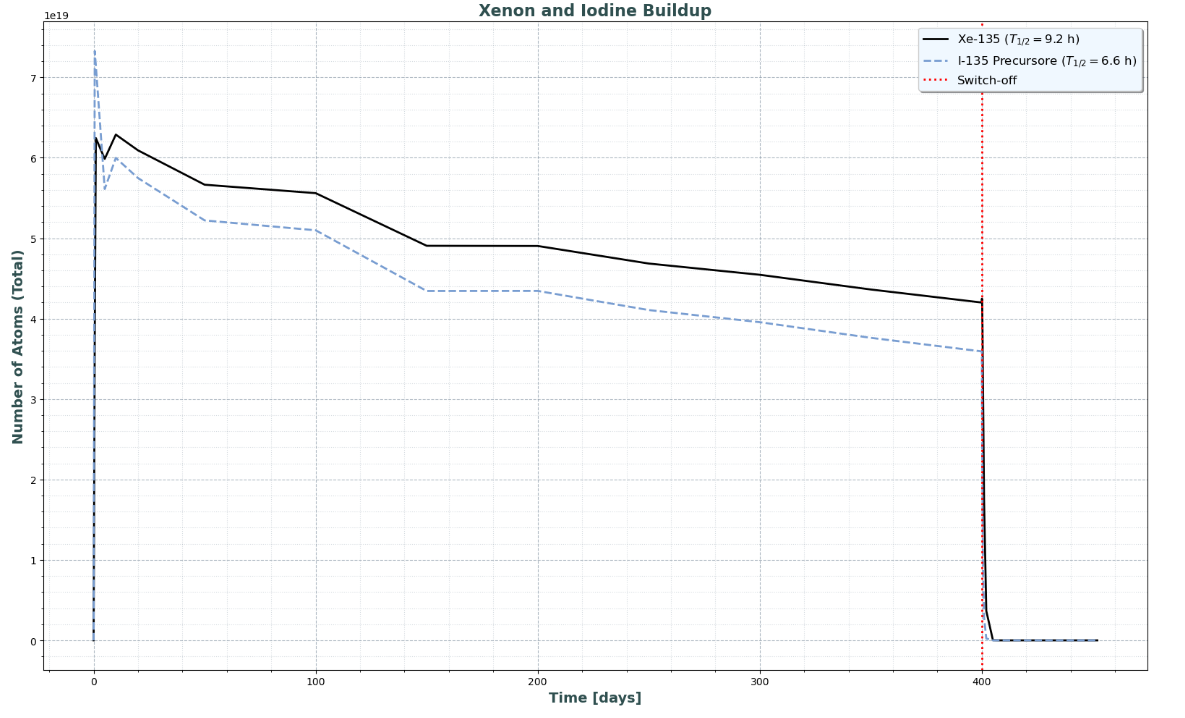
\includegraphics[height=0.75\textheight]{xenon-iodio.png} % Sostituisci con il nome del tuo file
    \end{center}
    \vfill
    \begin{flushleft}
        \scriptsize
        \textbf{Figura:} Andamento accoppiato delle densità atomiche dello Iodio-135 e dello Xenon-135 durante l'operatività nominale e nella fase successiva allo spegnimento del reattore (\textit{shutdown}). 
    \end{flushleft}
\end{frame}

% --- SLIDE 2: FOTO SULLO XENON ---
\begin{frame}{Evoluzione Temporale di $^{135}\text{I}$ e $^{135}\text{Xe}$}
    \begin{center}
        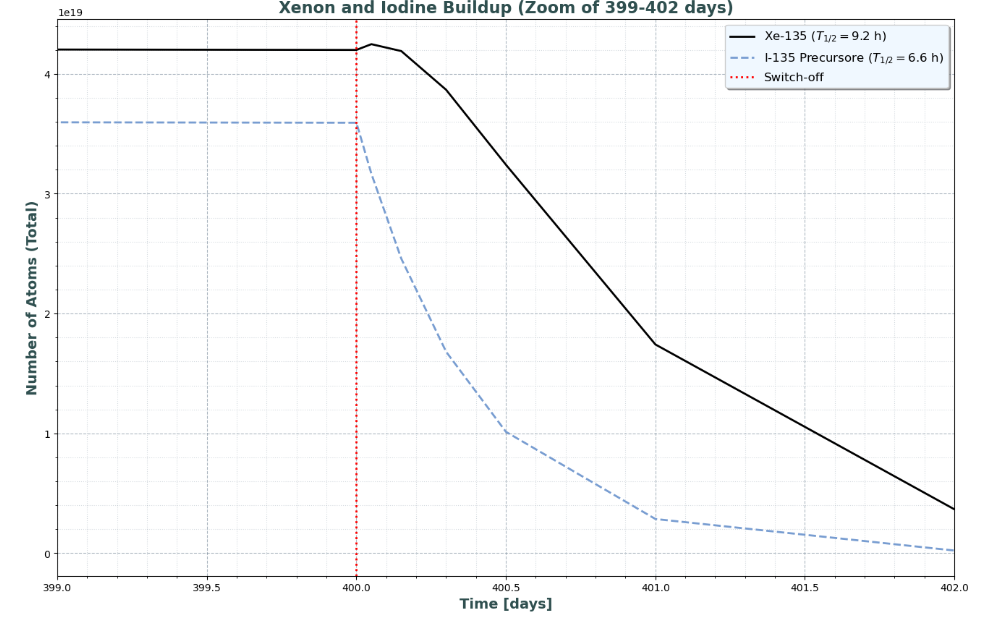
\includegraphics[height=0.75\textheight]{xenon-iodio-zoom.png} % Sostituisci con il nome del tuo file
    \end{center}
    \vfill
    \begin{flushleft}
        \scriptsize
        \textbf{Figura:} Il grafico mostra meglio l'insorgenza del picco di avvelenamento post spegnimento indotto dal disaccoppiamento dei tempi di dimezzamento dei due nuclidi.
    \end{flushleft}
\end{frame}

\begin{frame}{Evoluzione Temporale dello $^{135}\text{Xe}$ da simulazione}
    \begin{center}
        
\includegraphics[height=0.75\textheight]{xenon_transient_analysis.png} % Sostituisci con il nome del tuo file
    \end{center}
    \vfill
    \begin{flushleft}
        \scriptsize
        \textbf{Figura:} Il plot mostra l'evoluzione dello $^{135}\text{Xe}$ dopo lo spegnimento del reattore, evidenziando il picco di avvelenamento (xenon pit) e la successiva decrescita asintotica.
    \end{flushleft}
\end{frame}

% --- SLIDE 3: COMMENTO XENON ---
\begin{frame}{Analisi della Cinetica dello Xenon-135}
    \begin{itemize}
        \item \textbf{Fase Operativa (Equilibrio):} Durante il primo funzionamento, la produzione di $^{135}\text{I}$ è molto elevata, la sua presenza porta a produrre Xe, il quale diminuisce il flusso neutronico che fa diminuire la produzione di iodio in un circolo ripetitivo. 
        \item \textbf{Xenon Pit:} Allo spegnimento del reattore, il flusso neutronico crolla istantaneamente ($\phi \to 0$), annullando il termine di rimozione per cattura ($\sigma_{a,\text{Xe}}\phi N_{\text{Xe}} \to 0$) e la produzione di iodio.
        \item \textbf{Meccanismo del Picco:} Il $^{135}\text{I}$ accumulato nel core continua a decadere in $^{135}\text{Xe}$ con un tempo di dimezzamento inferiore ($T_{1/2} = 6.6$ h) rispetto a quello di distruzione dello Xenon ($T_{1/2} = 9.2$ h). Questa differenza genera un accumulo netto di veleno che raggiunge un massimo assoluto prima di decadere asintoticamente.
    \end{itemize}
\end{frame}

% --- SLIDE 4: FOTO SUL SAMARIO ---
\begin{frame}{Evoluzione Temporale di $^{149}\text{Pm}$ e $^{149}\text{Sm}$}
    \begin{center}
        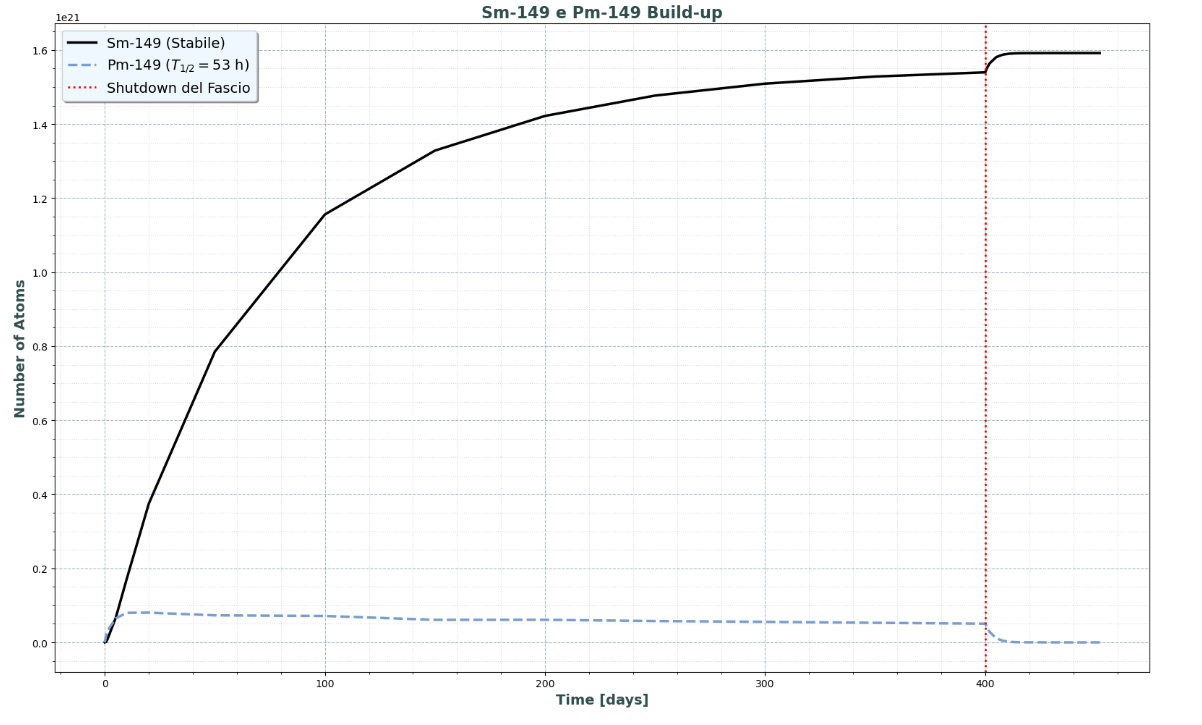
\includegraphics[height=0.65\textheight]{samario.png} % Sostituisci con il nome del tuo file
    \end{center}
    \begin{flushleft}
        \scriptsize
        \textbf{Figura:} Concentrazione del Promezio-149 e del Samario-149 in funzione del tempo di irraggiamento e dopo lo spegnimento. Si evidenzia il comportamento asintotico non decrescente del $^{149}\text{Sm}$ nella fase post-operativa dovuto alla stabilità intrinseca dell'isotopo.
    \end{flushleft}
\end{frame}

\begin{frame}{Evoluzione Temporale del $^{149}\text{Sm}$ da simulazione}
    \begin{center}
        
\includegraphics[height=0.75\textheight]{samarium_buildup_analysis.png} % Sostituisci con il nome del tuo file
    \end{center}
    \vfill
    \begin{flushleft}
        \scriptsize
        \textbf{Figura:} Il plot mostra l'evoluzione del $^{149}\text{Sm}$ dopo lo spegnimento del reattore, evidenziando il tempo necessario per raggiungere il plateau di avvelenamento residuo e la sua stabilità nel tempo.
    \end{flushleft}
\end{frame}

% --- SLIDE 5: COMMENTO SAMARIO ---
\begin{frame}{Analisi della Cinetica del Samario-149}
    \begin{itemize}
        \item \textbf{Indipendenza dal Flusso all'Equilibrio:} A differenza dello Xenon, la densità stazionaria di $^{149}\text{Sm}$ non dipende dal flusso neutronico totale $\phi$, poiché il flusso si semplifica analiticamente nel rapporto tra il tasso di produzione e quello di bruciamento .
        \item \textbf{Comportamento Post-Shutdown:} Quando il reattore viene spento, la distruzione per cattura neutronica si interrompe. Il $^{149}\text{Pm}$ presente nel core continua a decadere in $^{149}\text{Sm}$ con un tempo di dimezzamento di circa $53$ ore.
        \item \textbf{Stabilità Asintotica:} Poiché il $^{149}\text{Sm}$ è un nuclide stabile ($\lambda_{\text{Sm}} = 0$), la sua concentrazione post-spegnimento cresce fino a raggiungere un plateau costante senza subire successivi decadimenti. Questo livello di avvelenamento residuo rimane congelato nel core fino alla successiva riaccensione del sistema.
    \end{itemize}
\end{frame}

% --- SLIDE 6: FOTO POTENZA ---
\begin{frame}{Evoluzione della Potenza Termica del Core}
    \begin{center}
        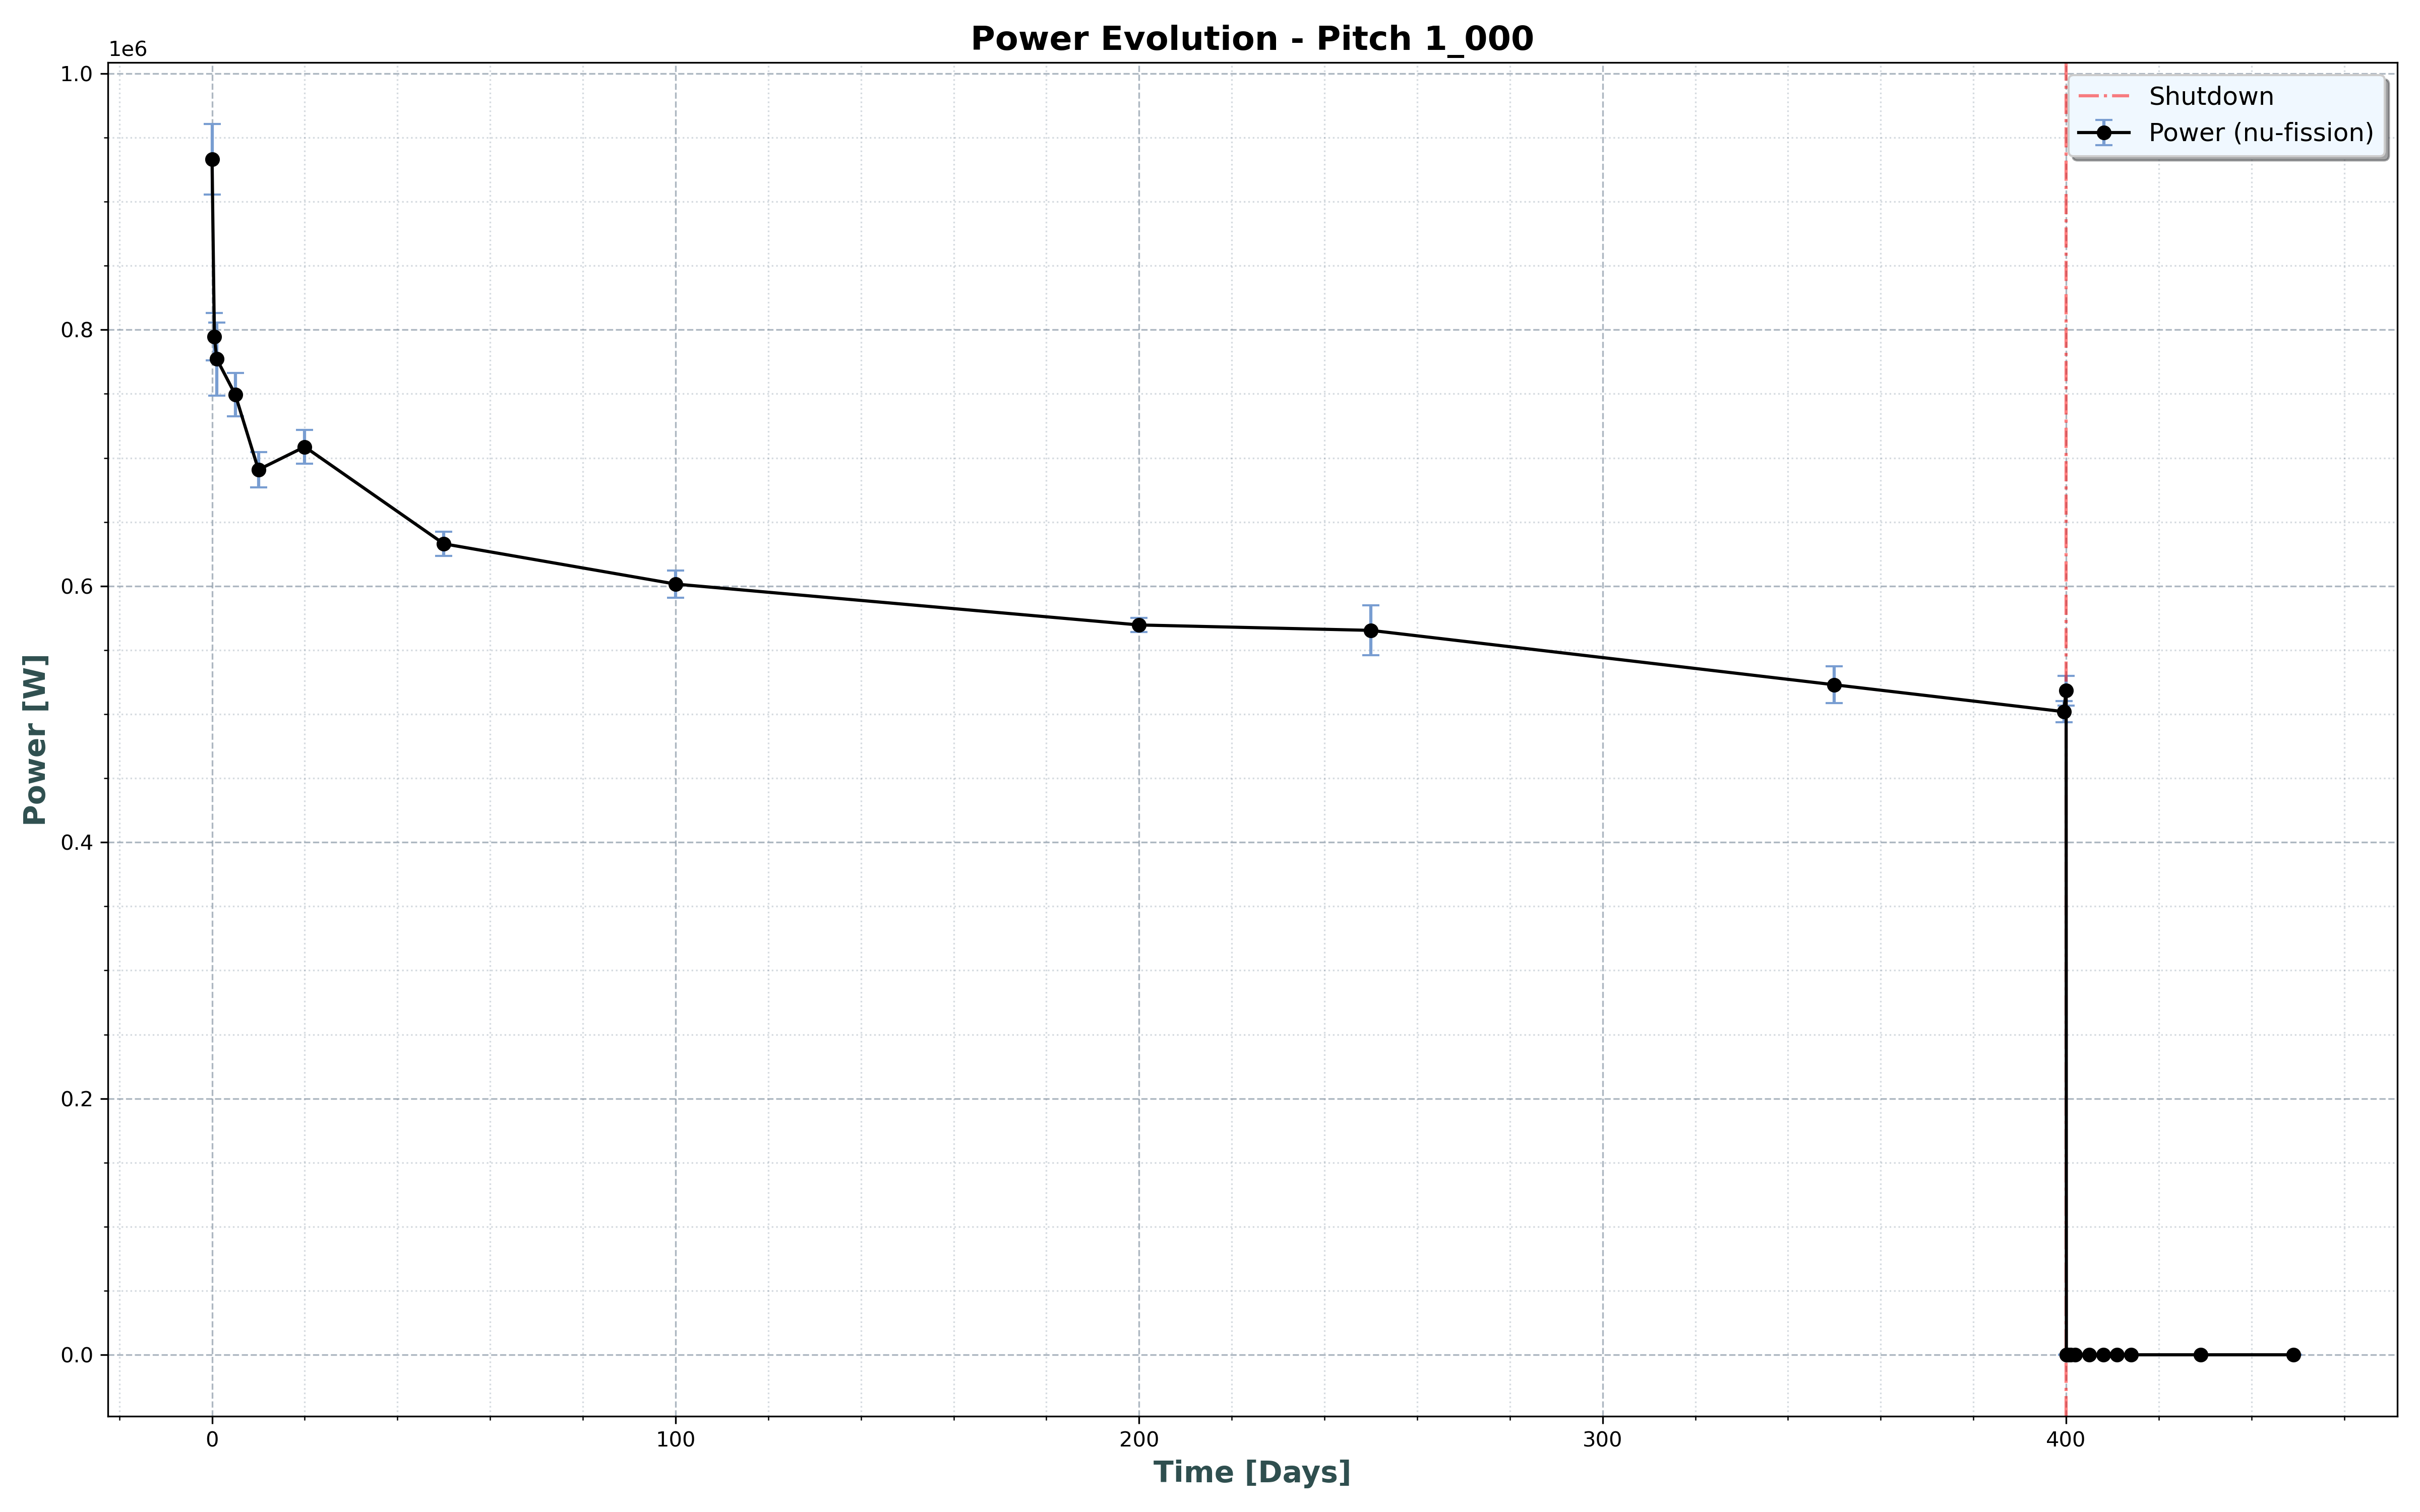
\includegraphics[height=0.75\textheight]{potenza.png} % Sostituisci con il nome del tuo file
    \end{center}
    \vfill
    \begin{flushleft}
        \scriptsize
        \textbf{Figura:} Profilo temporale della potenza termica globale espressa in W nel corso del ciclo di vita del combustibile. 
    \end{flushleft}
\end{frame}

% --- SLIDE 7: FOTO K_EFF ---
\begin{frame}{Evoluzione del Fattore di Moltiplicazione Effettivo ($k_{eff}$)}
    \begin{center}
        % Assicurati che keff.png sia presente nella cartella delle immagini
        
\includegraphics[height=0.75\textheight]{k_eff.png} 
    \end{center}
    \begin{flushleft}
        \scriptsize
        \textbf{Figura:} Andamento del fattore di moltiplicazione effettivo $k_{eff}$ in funzione dei giorni di operatività in piena potenza (HFP). Il tracciato documenta i margini di sicurezza legali e la stabilità complessiva del sistema rispetto all'avvelenamento e al consumo di fissile.
    \end{flushleft}
\end{frame}

% --- SLIDE 1: Formulazione e Operatori ---
\begin{frame}{Fondamento Matematico: L'Equazione del Trasporto}
Il bilancio neutronico stazionario è governato dall'equazione del trasporto:

\begin{alertblock}{Formulazione Operatoriale}
\begin{equation*}
\mathcal{M} \Phi(\vec{r}, E, \hat{\Omega}) = \frac{1}{k_{eff}} \mathcal{F} \Phi(\vec{r}, E, \hat{\Omega})
 \end{equation*}
\end{alertblock}

I due operatori descrivono i ratei fisici in competizione nel nocciolo:

\begin{itemize}
\item \textbf{$\mathcal{M}$ (Operatore di Migrazione/Distruzione):} Quantifica le perdite nette. Include le fughe geometriche (\textit{streaming}, $\hat{\Omega} \cdot \nabla \Phi$), le interazioni totali ($\Sigma_t \Phi$) e i ripopolamenti cinematici dovuti allo scattering (\textit{in-scattering}).
\item \textbf{$\mathcal{F}$ (Operatore di Produzione):} Quantifica la sorgente stazionaria, descrivendo l'emissione di nuovi neutroni rapidi indotta dal rateo di fissione integrale ($\chi \nu \Sigma_f \Phi$).
\end{itemize}
\end{frame}

% --- SLIDE 2: Spettro e Significato Fisico ---
\begin{frame}{Fondamento Matematico: Il Teorema di Krein-Rutman}
Riscrivendo l'equazione come $\mathcal{M}^{-1}\mathcal{F} \Phi = k_{eff} \Phi$, l'operatore $\mathcal{M}^{-1}\mathcal{F}$ mappa una generazione di neutroni in quella successiva. Essendo le densità atomiche e le sezioni d'urto quantità strettamente positive, tale operatore è \textbf{rigorosamente positivo}.

\begin{block}{Dominanza dell'Autovalore ($k_{eff}$)}
Per il \textbf{Teorema di Krein-Rutman}, un operatore integrale positivo garantisce l'esistenza di un autovalore fondamentale ($k_0 \equiv k_{eff}$) reale, positivo e \textbf{maggiore in modulo} di tutti gli altri autovalori dello spettro ($|k_0| > |k_n|$).
\end{block}

\begin{alertblock}{Significato Fisico dell'Autofunzione ($\Phi_0$)}
Solo all'autovalore dominante $k_{eff}$ è associata un'autofunzione $\Phi_0$ \textbf{ovunque definita positiva}. Le armoniche di ordine superiore presentano inevitabilmente dei nodi (flussi negativi, fisicamente impossibili in stazionario).
\end{alertblock}
\end{frame}

\end{document}